\documentclass[aspectratio=169,10pt]{beamer}
\usepackage[utf8]{vietnam}
\usepackage{amsmath,amssymb}
\usepackage{booktabs,tabularx,array}
\usepackage{graphicx}
\usepackage{tikz}
\usetikzlibrary{shapes.geometric,arrows.meta,positioning}

\usetheme{Madrid}
\definecolor{ptitred}{RGB}{180,25,35}
\definecolor{ptitnavy}{RGB}{20,45,90}
\setbeamercolor{palette primary}{bg=ptitnavy,fg=white}
\setbeamercolor{palette secondary}{bg=ptitred,fg=white}
\setbeamercolor{palette tertiary}{bg=ptitnavy,fg=white}
\setbeamercolor{structure}{fg=ptitnavy}
\setbeamercolor{block title}{bg=ptitnavy,fg=white}
\setbeamercolor{block body}{bg=blue!4,fg=black}
\setbeamercolor{alerted text}{fg=ptitred}
\setbeamertemplate{navigation symbols}{}
\setbeamertemplate{itemize items}[circle]

\title[Xử lý ảnh \& CNN trên HAM10000]{\textbf{Đánh Giá Tác Động Của Xử Lý Ảnh Cổ Điển Lên Phân Loại Tổn Thương Da HAM10000 Bằng Mạng Tích Chập}}
\subtitle{Đồ án Học phần Xử lý Ảnh -- Khoa Trí tuệ Nhân tạo, PTIT}
\author[Nhóm Đồ án XLA]{\small Nguyễn Trung Nam (B23DCVT299) \quad Phan Nguyễn Việt Dũng (B23DCCN210)\\[2pt] Lê Duy Anh (B23DCCN026) \quad Đinh Khánh Sơn (B23DCDT223) \quad Đào Phạm Bích Ngọc (B23DCVT308)}
\institute[PTIT]{Học viện Công nghệ Bưu chính Viễn thông}
\date{Tháng 11 / 2026}

\begin{document}

% Slide 1
\begin{frame}
\titlepage
\end{frame}

% Slide 2
\begin{frame}{1. Bài toán, Động cơ \& Câu hỏi Nghiên cứu}
\begin{columns}[T,onlytextwidth]
\begin{column}{0.54\textwidth}
\begin{block}{Triết lý thực nghiệm xuyên suốt}
\textbf{Không săn điểm SOTA} -- tập trung \textbf{Lập luận $\rightarrow$ Thực nghiệm kiểm soát biến $\rightarrow$ Đánh giá trung thực} (kết quả âm vẫn có giá trị khoa học).
\end{block}
\vspace{2pt}
\begin{itemize}
    \item \textbf{Bài toán:} Phân loại 7 lớp bệnh da trên tập ảnh soi da lâm sàng \textbf{HAM10000} ($10\,015$ ảnh $600{\times}450$).
    \item \textbf{Thách thức:} Mất cân bằng lớp $58{,}3\times$; nhiều ảnh chung \texttt{lesion\_id}; nhiễu thiết bị (viền đen, lóa gel, lông, tương phản thấp).
    \item \textbf{Kiến thức học phần tích hợp:} Chương 3 (nâng cao ảnh), Chương 4 (hệ màu), Chương 5 (Otsu/Sobel), Chương 7 (hình thái học), Chương 8 (CNN \& Grad-CAM).
\end{itemize}
\end{column}
\begin{column}{0.43\textwidth}
\begin{block}{4 Câu hỏi nghiên cứu (RQ)}
\footnotesize
\begin{enumerate}
    \item \textbf{RQ1 (EDA):} Có những lỗi chất lượng ảnh nào có bằng chứng thống kê \& liên hệ lỗi CNN?
    \item \textbf{RQ2 (Ablation):} Xử lý ảnh cổ điển có tạo $\Delta$ macro-F1 vượt dao động giữa 3 seed?
    \item \textbf{RQ3 (4 tầng):} Nếu F1 toàn tập không tăng, tiền xử lý tác động ở tầng nào?
    \item \textbf{RQ4 (Pipeline):} Kết hợp nhiều bước \& chọn kiến trúc CNN tối ưu ra sao?
\end{enumerate}
\end{block}
\end{column}
\end{columns}
\end{frame}

% Slide 3
\begin{frame}{2.1 Dữ liệu HAM10000 \& Đặc thù Miền Ảnh Dermoscopy}
\begin{columns}[T,onlytextwidth]
\begin{column}{0.55\textwidth}
\centering
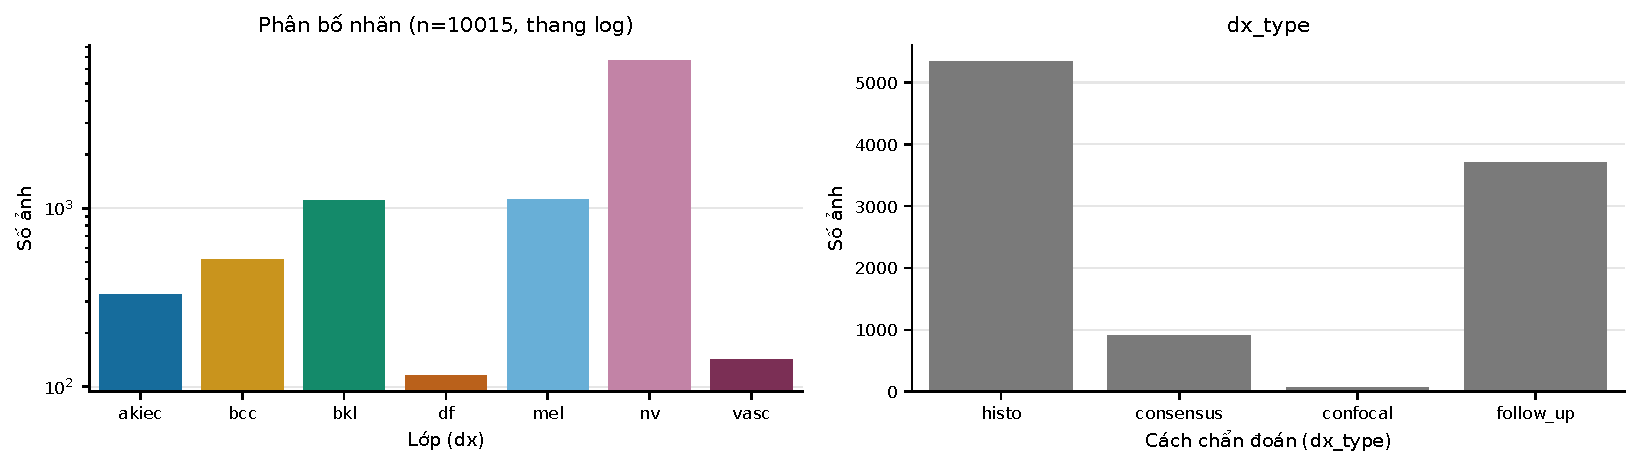
\includegraphics[width=\linewidth]{figures/class_distribution.pdf}
\end{column}
\begin{column}{0.42\textwidth}
\footnotesize
\begin{itemize}
    \item \textbf{Quy mô:} $10\,015$ ảnh RGB ($600{\times}450$) từ $7\,470$ \texttt{lesion\_id}.
    \item \textbf{Mất cân bằng 58,3$\times$:} \texttt{nv} chiếm $66{,}95\%$ ($6\,705$ ảnh), \texttt{df} chỉ $115$ ảnh $\Rightarrow$ luôn đoán \texttt{nv} đạt Acc $66{,}9\%$ nhưng \alert{Macro-F1 chỉ $0{,}1145$}.
    \item \textbf{Đa ảnh/lesion:} $26{,}2\%$ lesion có $2\text{--}6$ ảnh ($44{,}9\%$ số ảnh) $\Rightarrow$ bắt buộc chia theo \texttt{lesion\_id}.
    \item \textbf{Nguồn nhãn:} $100\%$ ảnh \texttt{follow\_up} ($3\,704$ ảnh) thuộc lớp \texttt{nv} $\Rightarrow$ nguy cơ shortcut nguồn chụp.
    \item \textbf{Lưu ý miền dữ liệu:} Ảnh soi da áp sát (\emph{dermoscopy}), khác miền với ảnh điện thoại.
\end{itemize}
\end{column}
\end{columns}
\end{frame}

% Slide 4
\begin{frame}{2.2 Phân tích Chất lượng Ảnh (EDA): 7 Chỉ số Định lượng}
\begin{columns}[T,onlytextwidth]
\begin{column}{0.54\textwidth}
\centering
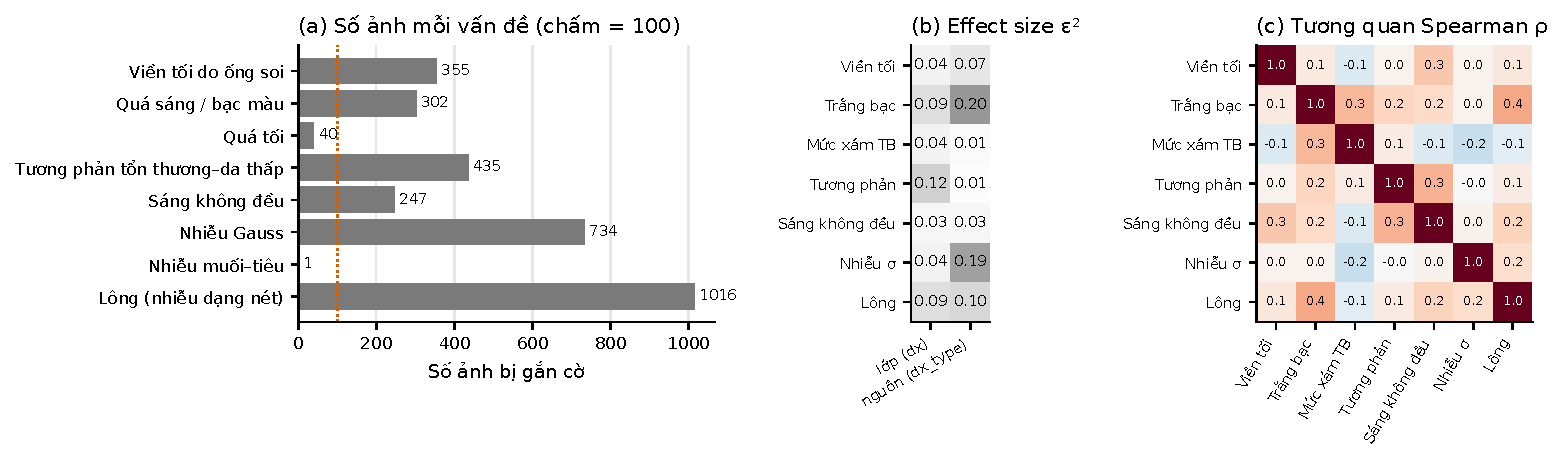
\includegraphics[width=\linewidth]{figures/eda_summary.pdf}
\end{column}
\begin{column}{0.43\textwidth}
\scriptsize
\begin{tabular}{lrr}
\toprule
\textbf{Vấn đề (Ch.3, 4, 5, 7)} & \textbf{Số ảnh} & \textbf{Tỉ lệ} \\
\midrule
1. Lông (Black-hat $17{\times}17$) & $1\,016$ & $10{,}1\%$ \\
2. Nhiễu Gauss ($\sigma > 2{,}16$) & $734$ & $7{,}3\%$ \\
3. Tương phản thấp ($<20$) & $435$ & $4{,}3\%$ \\
4. Viền tối ống soi ($>1\%$) & $355$ & $3{,}5\%$ \\
5. Quá sáng bạc màu ($>10\%$) & $302$ & $3{,}0\%$ \\
6. Sáng không đều ($>38$) & $247$ & $2{,}5\%$ \\
\midrule
Quá tối / Muối--tiêu & $40$ / $1$ & \alert{Bác bỏ} \\
\bottomrule
\end{tabular}
\vspace{4pt}
\begin{itemize}
    \item Kiểm chứng bộ đo bằng nhiễu tổng hợp: sai số $<0{,}1$ mức xám $\Rightarrow$ bác bỏ muối--tiêu là kết luận thực chứng.
    \item $|\rho_{\text{Spearman}}| \le 0{,}40$: 7 chỉ số độc lập, không đo trùng.
\end{itemize}
\end{column}
\end{columns}
\end{frame}

% Slide 5
\begin{frame}{2.3 Chuẩn bị Dữ liệu Chống Rò rỉ \& Cân bằng Lớp WRS}
\begin{columns}[T,onlytextwidth]
\begin{column}{0.48\textwidth}
\footnotesize
\begin{block}{Chia tập cố định theo \texttt{lesion\_id} (seed 42)}
\texttt{StratifiedGroupKFold} 2 tầng (0 lesion trùng lặp):
\begin{itemize}
    \item \textbf{Train\_fit:} $6\,408$ ảnh ($4\,779$ lesion -- $63{,}98\%$)
    \item \textbf{Validation:} $1\,603$ ảnh ($1\,196$ lesion -- $16{,}01\%$)
    \item \textbf{Test:} $2\,004$ ảnh ($1\,495$ lesion -- $20{,}01\%$)
\end{itemize}
\end{block}
\vspace{3pt}
\begin{itemize}
    \item \textbf{Metadata:} Điền \texttt{age} thiếu (57 ảnh) bằng median tập train ($50{,}0$), giữ nguyên toàn bộ ảnh hợp lệ.
    \item \textbf{Tránh bù 2 lần:} Dùng \texttt{WeightedRandomSampler} ($w_i = 1/n_{y_i}$, mỗi lớp $\approx 14{,}29\%$/epoch) + \texttt{CrossEntropyLoss} \emph{không} class weights.
\end{itemize}
\end{column}
\begin{column}{0.49\textwidth}
\centering
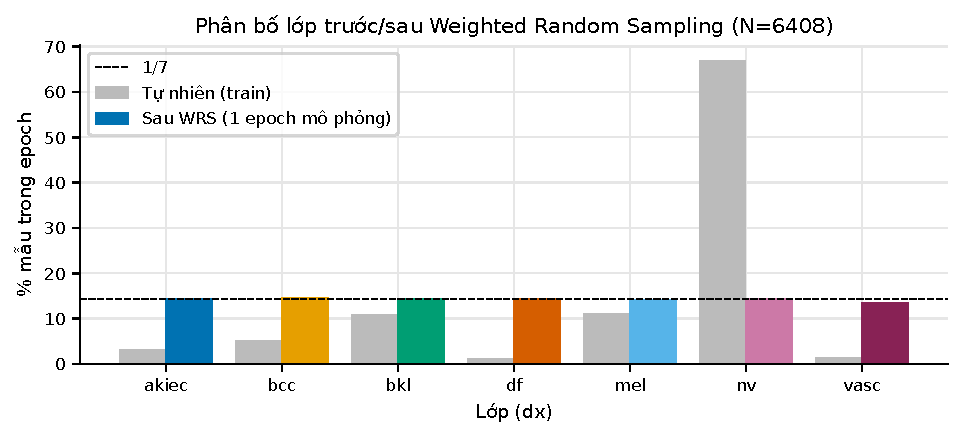
\includegraphics[width=\linewidth]{figures/wrs_distribution.pdf}
\end{column}
\end{columns}
\end{frame}

% Slide 6
\begin{frame}{2.4 Baseline \& Khảo sát 3 Kiến trúc CNN (3 Seed: 42, 43, 44)}
\begin{columns}[T,onlytextwidth]
\begin{column}{0.52\textwidth}
\centering
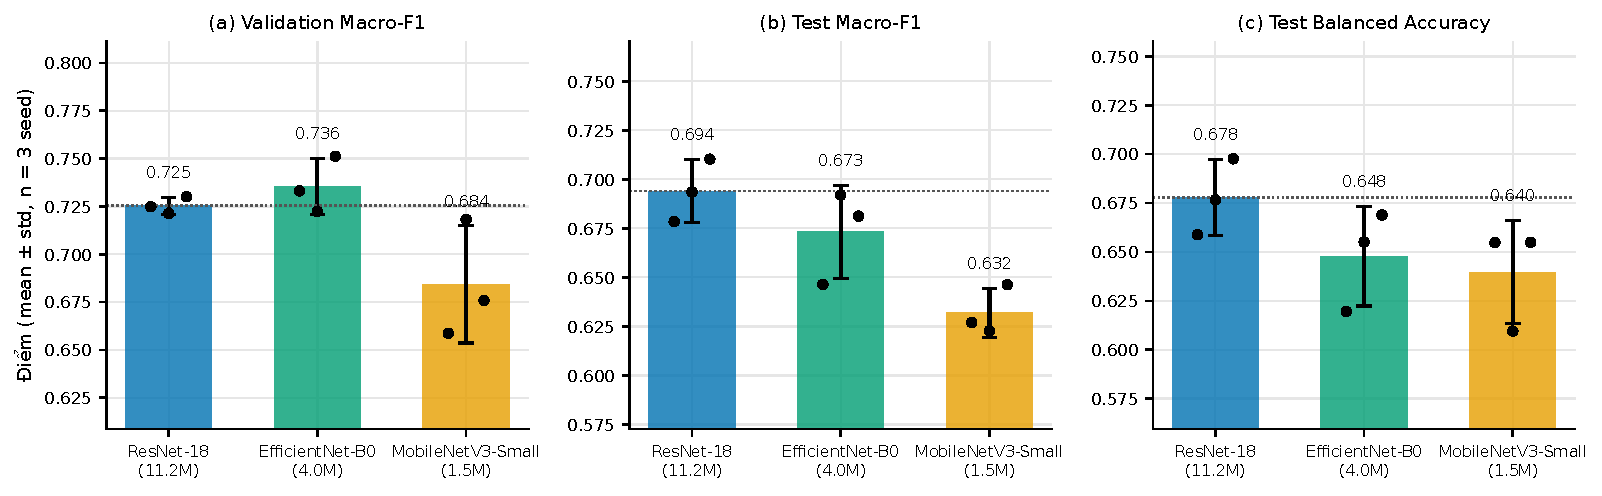
\includegraphics[width=\linewidth]{figures/backbone_comparison.pdf}
\end{column}
\begin{column}{0.45\textwidth}
\scriptsize
\begin{tabular}{lccc}
\toprule
\textbf{Kiến trúc} & \textbf{Tham số} & \textbf{Val F1} & \textbf{Test F1} \\
\midrule
\textbf{ResNet-18} & $11{,}18$M & $0{,}7254$ & $\mathbf{0{,}6941}$ \\
EfficientNet-B0 & $4{,}02$M & $0{,}7355$ & $0{,}6732$ \\
MobileNetV3-S & $1{,}53$M & $0{,}6842$ & $0{,}6320$ \\
\bottomrule
\end{tabular}
\vspace{3pt}
\footnotesize
\begin{itemize}
    \item \textbf{ResNet-18 Baseline:} Val F1 $= 0{,}7254 \pm 0{,}0044$; Test F1 $= \mathbf{0{,}6941 \pm 0{,}0160}$; bAcc $= 0{,}6777 \pm 0{,}0194$; Acc $= 0{,}8315 \pm 0{,}0032$.
    \item Cấu hình đóng băng: $224{\times}224$, AdamW $\text{lr}=10^{-4}$, batch $32$, $20$ epoch, chọn epoch theo \texttt{val} F1.
    \item Giữ cố định \textbf{ResNet-18} cho toàn bộ 16 thí nghiệm mục 2.5 để kiểm soát biến tuyệt đối \& trích Grad-CAM \texttt{layer4}.
\end{itemize}
\end{column}
\end{columns}
\end{frame}

% Slide 7
\begin{frame}{2.5a Ablation Nhóm 1: Khử Nhiễu Gauss \& Tăng Tương Phản}
\begin{columns}[T,onlytextwidth]
\begin{column}{0.52\textwidth}
\centering
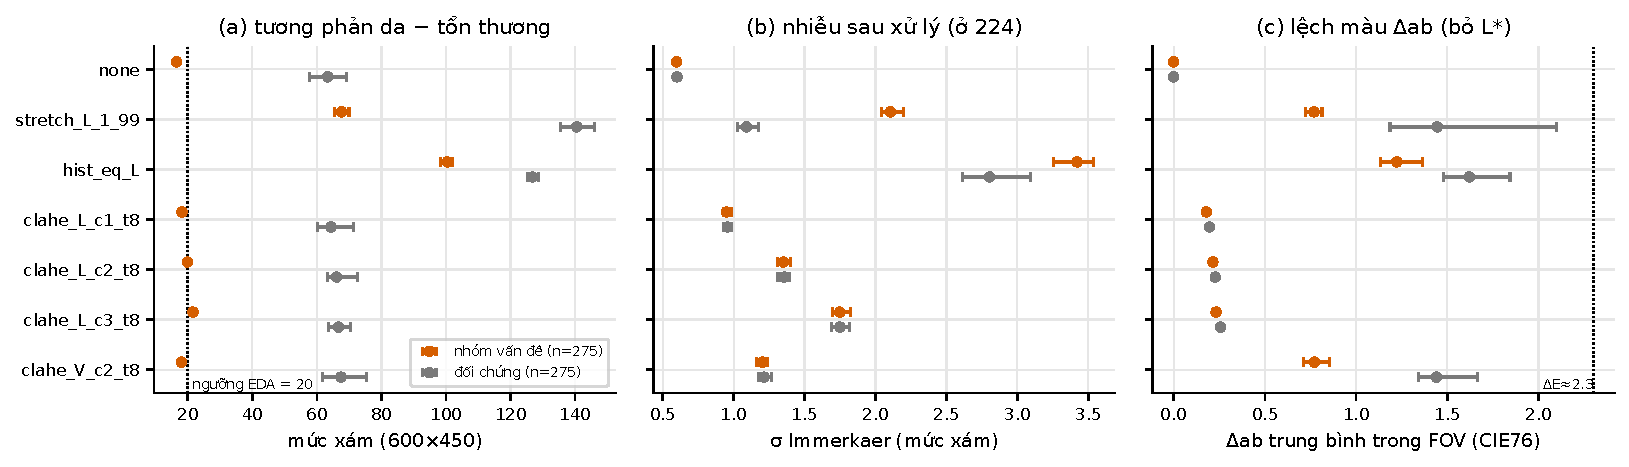
\includegraphics[width=\linewidth]{figures/contrast_metrics.pdf}
\end{column}
\begin{column}{0.45\textwidth}
\scriptsize
\begin{tabular}{lccl}
\toprule
\textbf{Cấu hình} & \textbf{Val F1} & \textbf{Test F1} & \textbf{Kết luận} \\
\midrule
\texttt{baseline} & $0{,}7254$ & $0{,}6941$ & Đối chứng \\
\texttt{gauss3} & $0{,}7238$ & $0{,}6422$ & tệ hơn rõ \\
\texttt{median3} & $0{,}7294$ & $0{,}6833$ & không khác biệt rõ \\
\texttt{median5} & $0{,}7196$ & $0{,}6720$ & không khác biệt rõ \\
\texttt{stretch\_L\_1\_99} & $0{,}6920$ & $0{,}6154$ & \alert{\textbf{Tệ hơn rõ}} \\
\texttt{hist\_eq\_L} & $0{,}6472$ & $0{,}5834$ & \alert{\textbf{Tệ hơn rõ}} \\
\texttt{clahe\_L\_c2\_t8} & $0{,}7261$ & $0{,}6706$ & không khác biệt rõ \\
\bottomrule
\end{tabular}
\vspace{3pt}
\footnotesize
\begin{itemize}
    \item Resize $600{\rightarrow}224$ đã hạ $\sigma$ nhiễu; \texttt{median5} xóa $75\%$ chi tiết Laplacian tổn thương.
    \item \alert{\texttt{hist\_eq\_L} \& \texttt{stretch\_L\_1\_99}} nhân nhiễu $\times 3{,}5\text{--}5{,}5$ và làm lệch màu $\Delta E_{76} = 14\text{--}22$ trên $95{,}7\%$ ảnh thường!
\end{itemize}
\end{column}
\end{columns}
\end{frame}

% Slide 8
\begin{frame}{2.5b Ablation Nhóm 2: Đại trà vs Có điều kiện (Lông, Viền, Sáng)}
\begin{columns}[T,onlytextwidth]
\begin{column}{0.42\textwidth}
\centering
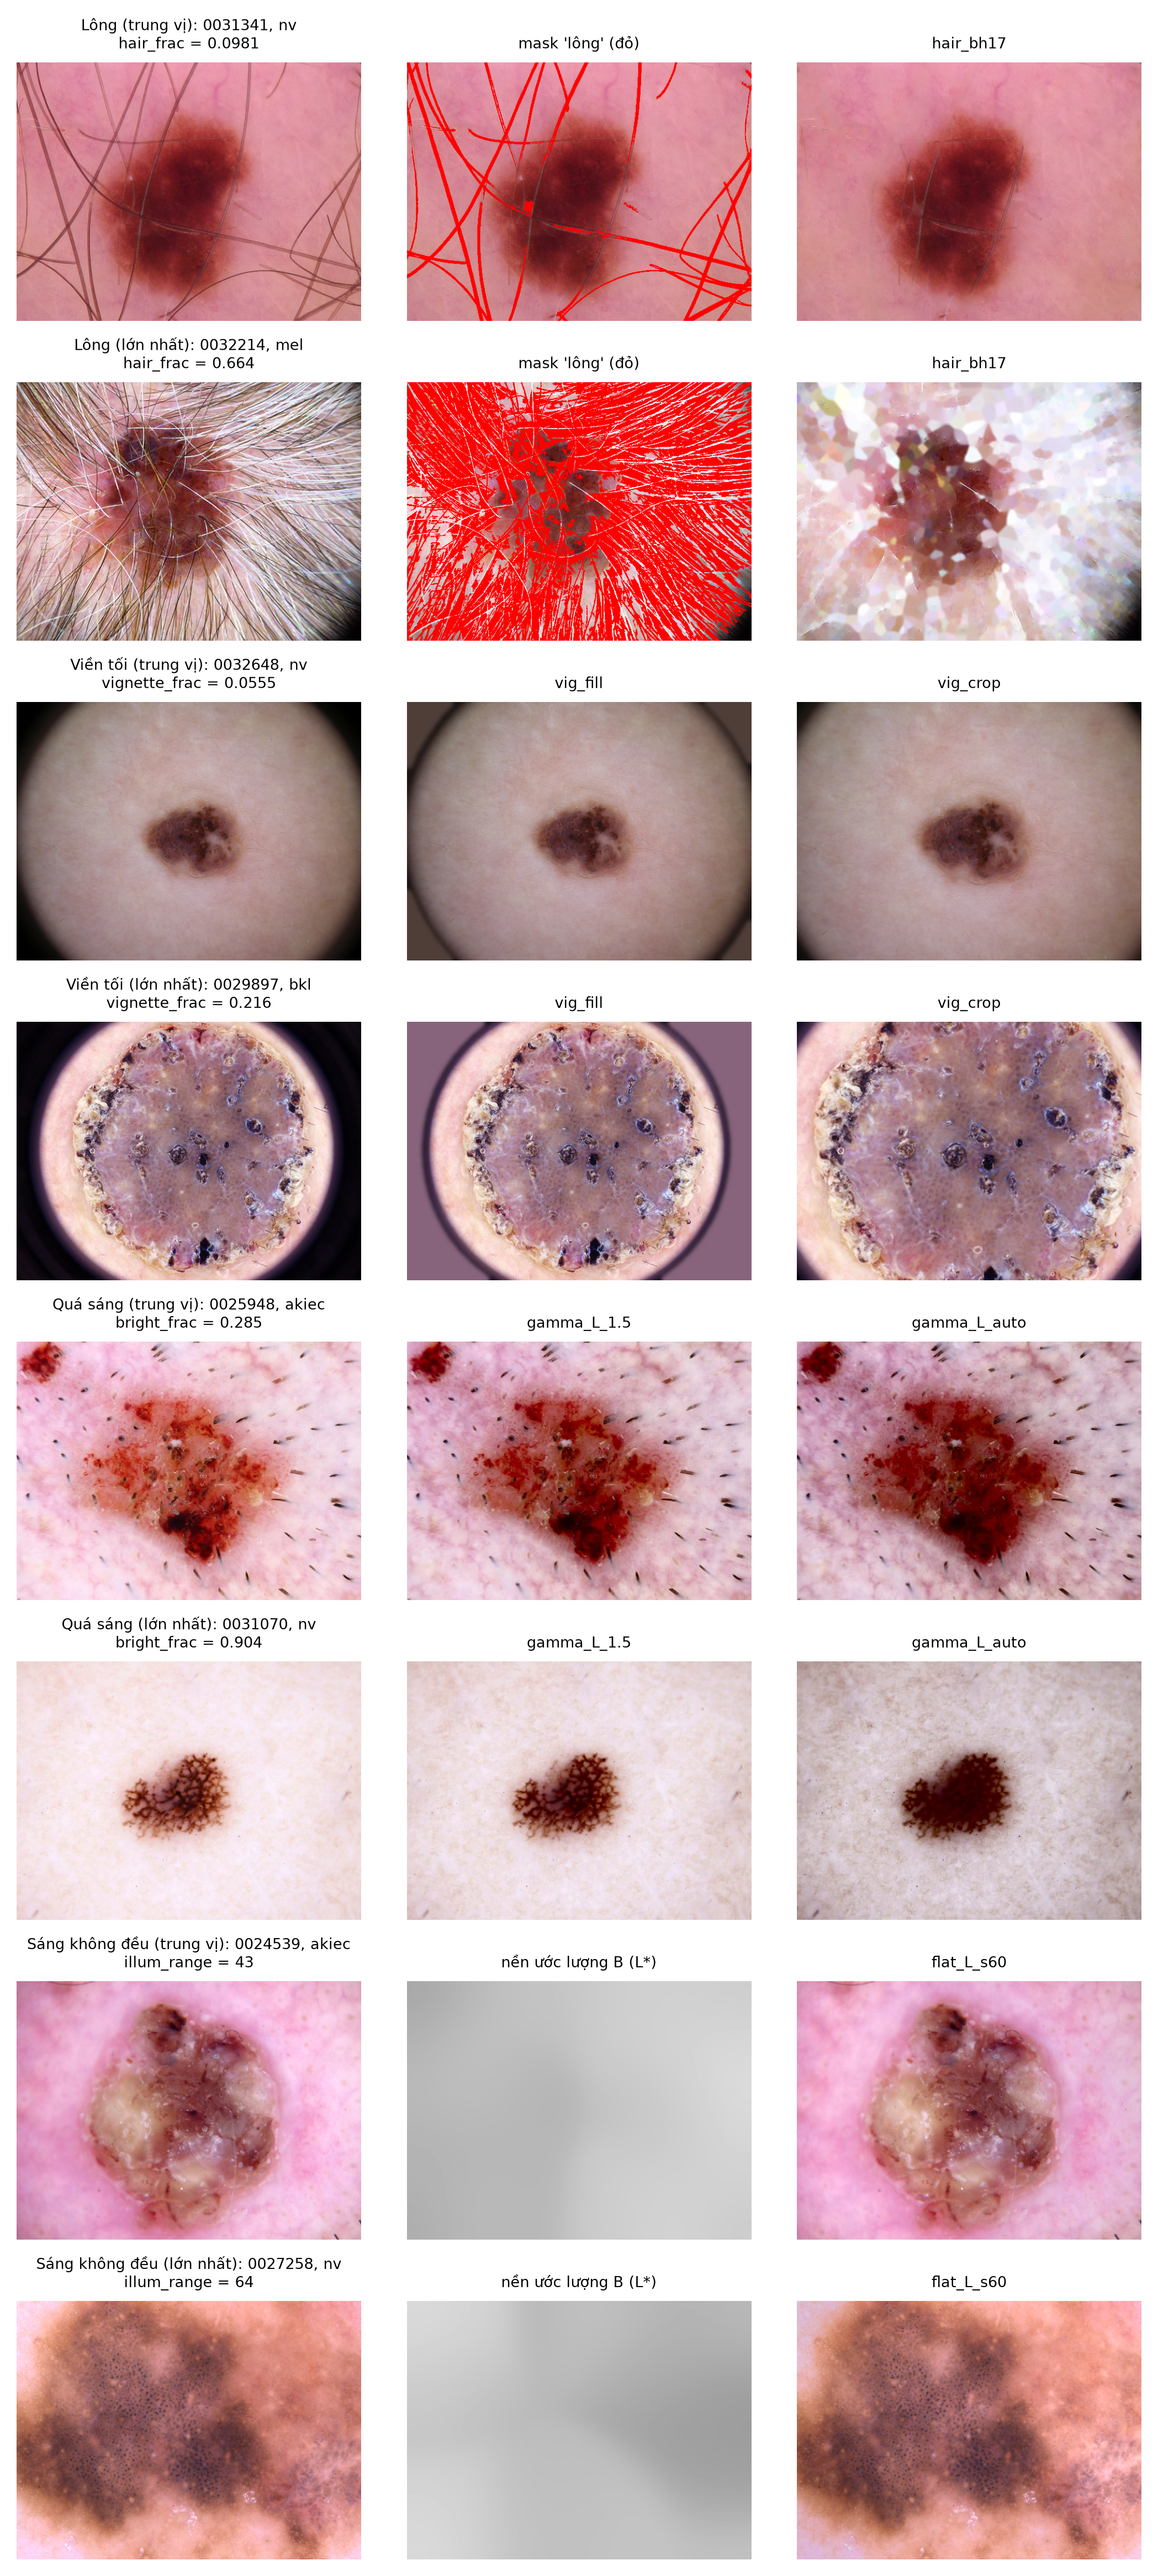
\includegraphics[height=0.72\textheight,keepaspectratio]{figures/artifacts_before_after.png}
\end{column}
\begin{column}{0.55\textwidth}
\scriptsize
\begin{block}{Bài học lớn nhất: Xử lý Đại trà vs Có điều kiện (\texttt{\_cond})}
\begin{itemize}
    \item \textbf{Bản \texttt{\_cond}} để nguyên \textbf{100\% ảnh bình thường} ($\Delta E_{76} = 0$).
    \item \alert{\texttt{hair\_bh17} (áp đại trà)} sửa nhầm $92\%$ ảnh không lông, xóa trung vị \textbf{8.9\%} diện tích tổn thương \texttt{mel} (vs 2.5\% ở \texttt{nv}) $\Rightarrow$ giảm điểm cả 3/3 seed!
    \item Ca lỗi kinh điển: \textbf{lông bạc/trắng} bị black-hat bắt ngược khe da tối, gây loang mảng sau inpainting.
\end{itemize}
\end{block}
\vspace{2pt}
\centering
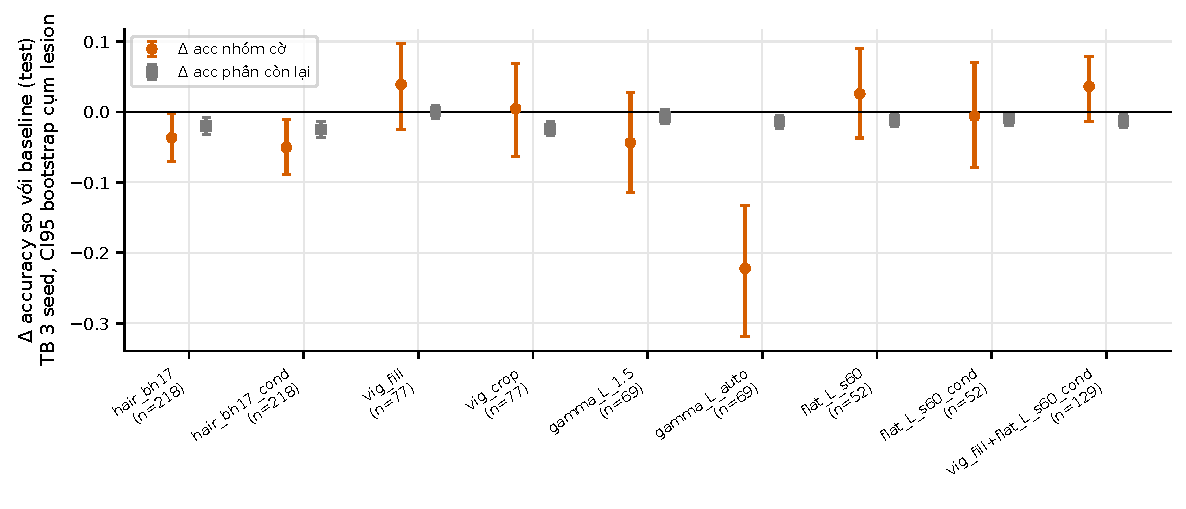
\includegraphics[height=0.33\textheight,keepaspectratio]{figures/subgroup_delta.pdf}
\end{column}
\end{columns}
\end{frame}

% Slide 9
\begin{frame}{Tổng hợp 16 Cấu hình Tiền xử lý trên ResNet-18 (NVIDIA L40S)}
\centering
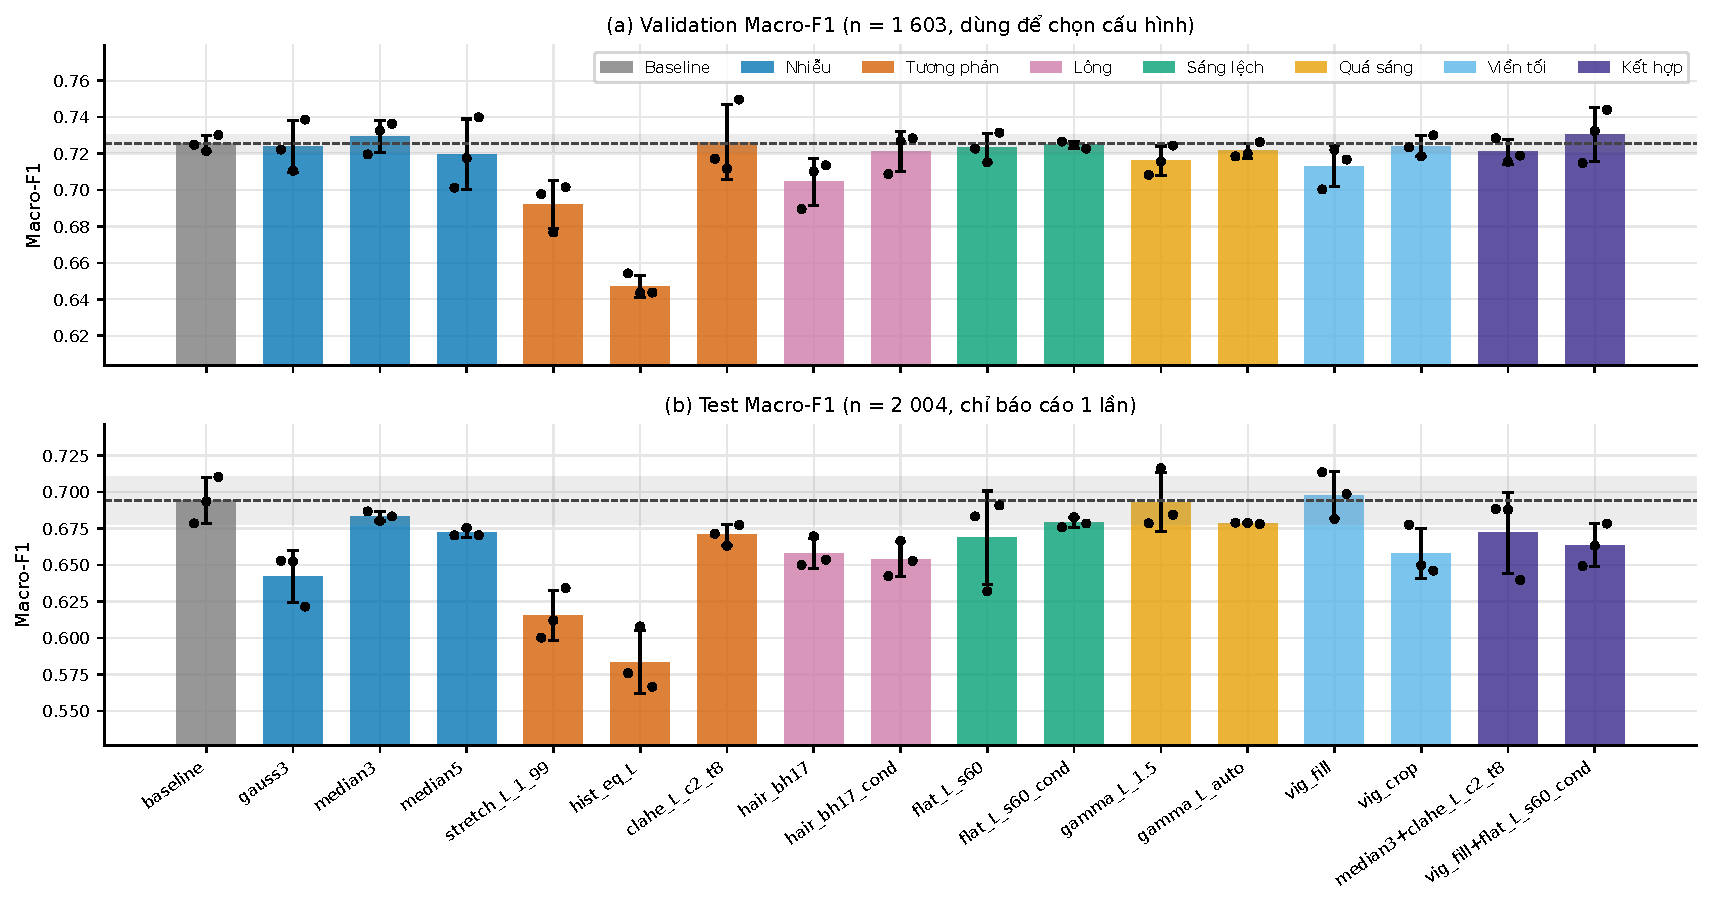
\includegraphics[height=0.61\textheight,keepaspectratio]{figures/all16_macro_f1.pdf}\par
\vspace{3pt}
\footnotesize
\textbf{Kết luận RQ2 \& RQ4:} \alert{0/16 cấu hình} (kể cả 2 cấu hình kết hợp \texttt{median3+clahe} và \texttt{vig\_fill+flat\_cond}) vượt chuẩn ``tốt hơn rõ'' trên Validation ($|\Delta| > \text{std}_{\text{base}}$, CI95 loại 0, 3/3 seed dương).
\end{frame}

% Slide 10
\begin{frame}{2.5c Giải mã Nghịch lý qua 4 Tầng Phân tích (RQ3)}
\begin{columns}[T,onlytextwidth]
\begin{column}{0.48\textwidth}
\footnotesize
\begin{enumerate}
    \item \textbf{Tầng A (Ảnh):} Triệt tiêu $92\%\text{--}100\%$ cờ EDA mục tiêu, nhưng CNN fine-tune toàn mạng có \texttt{BatchNorm} đã tự bù biến thiên sáng nhẹ.
    \item \textbf{Tầng B (Đổi nhãn):} Hai seed baseline tự bất đồng $\approx 11\%\text{--}12\%$ ảnh; các bản \texttt{\_cond} nằm sát mức nền này.
    \item \textbf{Tầng C (Stress Test):} Khi suy giảm ngoại lai nặng (viền đen lớn, lông dày, nhiễu cao), tiền xử lý \textbf{giúp phục hồi rõ rệt F1}!
    \item \textbf{Tầng D (Grad-CAM \texttt{layer4}):} Giảm chú ý vào viền/lông ở biên, giữ ổn định trọng tâm tổn thương.
\end{enumerate}
\end{column}
\begin{column}{0.50\textwidth}
\centering
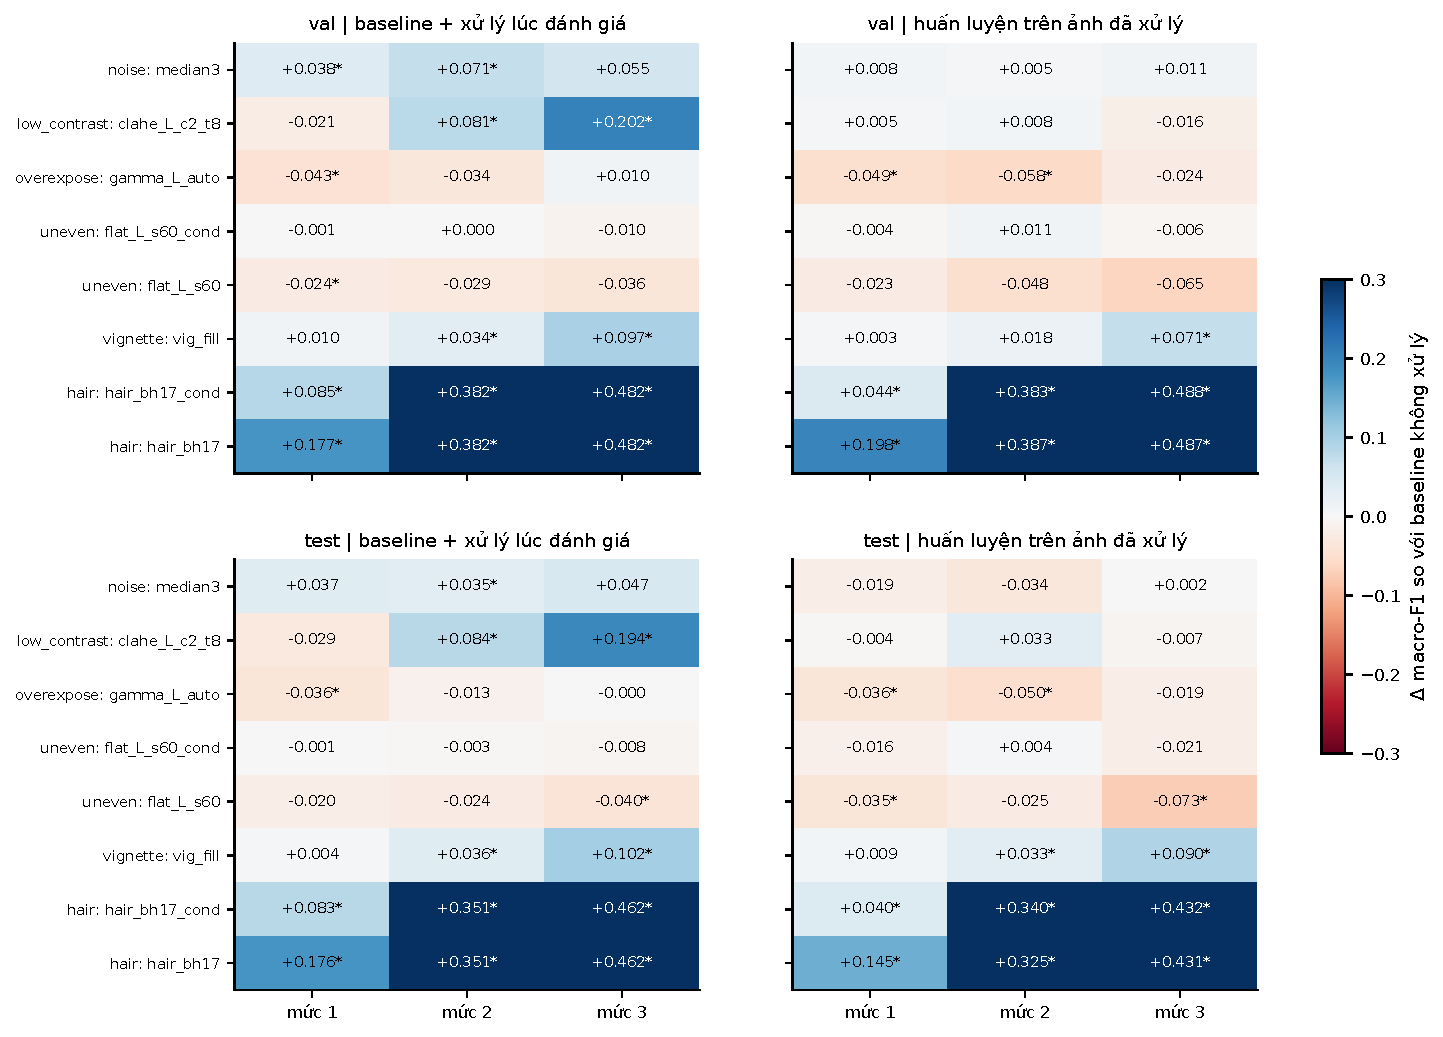
\includegraphics[width=0.96\linewidth]{figures/impact_c2_stress.pdf}
\end{column}
\end{columns}
\end{frame}

% Slide 11
\begin{frame}{2.6 -- 2.7 Pipeline Đề xuất Hai Nhánh \& Đóng băng Mô hình Cuối}
\centering
\begin{tikzpicture}[node distance=0.8cm and 1.1cm, >=Latex, every node/.style={font=\footnotesize}]
\node[draw, rounded corners, fill=gray!15, minimum width=2.8cm, minimum height=1.1cm, align=center] (in) {\textbf{Ảnh Dermoscopy}\\RGB $600{\times}450$};
\node[draw, rounded corners, fill=orange!15, minimum width=5.6cm, minimum height=1.3cm, align=center, above right=0.25cm and 1.2cm of in] (qc) {\textbf{Nhánh (A): Kiểm tra Chất lượng (QC)}\\6 bộ dò Ch.3--7 $\rightarrow$ Gắn cờ cảnh báo độ tin cậy\\(+ Minh họa bước có điều kiện \texttt{vig\_fill}, \texttt{flat\_cond})};
\node[draw, rounded corners, fill=blue!12, minimum width=5.6cm, minimum height=1.3cm, align=center, below right=0.25cm and 1.2cm of in] (cnn) {\textbf{Nhánh (B): Phân loại CNN (ResNet-18)}\\Ảnh gốc $\rightarrow$ Resize $224$ $\rightarrow$ Normalize ImageNet\\$\rightarrow$ Dự đoán 7 lớp + Bản đồ nhiệt Grad-CAM};
\draw[->, thick] (in.east) -- ++(0.45,0) |- (qc.west);
\draw[->, thick] (in.east) -- ++(0.45,0) |- (cnn.west);
\end{tikzpicture}
\vspace{6pt}
\begin{block}{Lý do thiết kế từ thực nghiệm}
\footnotesize
\begin{itemize}
    \item Không ép ảnh qua biến đổi pixel cố định ở nhánh (B) vì 0/16 cấu hình giúp tăng F1 trên dữ liệu thật và có nguy cơ làm mất tín hiệu màu/sắc tố.
    \item Đưa tri thức Chương 3--7 vào \textbf{Nhánh (A) QC} để phát hiện ảnh sáng lệch / quá sáng (nhóm có lỗi thực tế cao hơn kỳ vọng) và hỗ trợ giải thích trực quan.
\end{itemize}
\end{block}
\end{frame}

% Slide 12
\begin{frame}{2.8 Phân tích Lỗi Chuyên sâu của Mô hình Cuối}
\begin{columns}[T,onlytextwidth]
\begin{column}{0.46\textwidth}
\centering
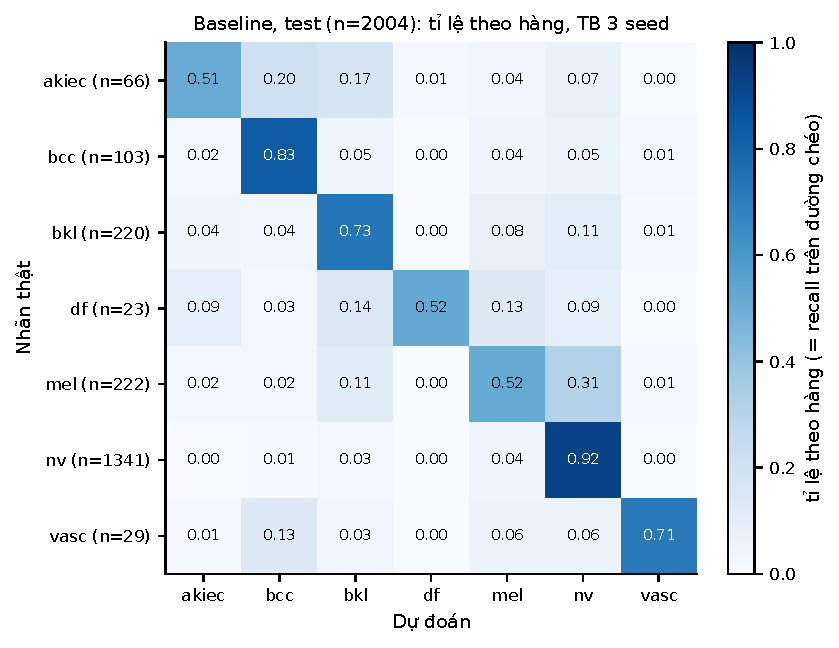
\includegraphics[width=0.92\linewidth]{figures/confusion_test.pdf}
\end{column}
\begin{column}{0.52\textwidth}
\centering
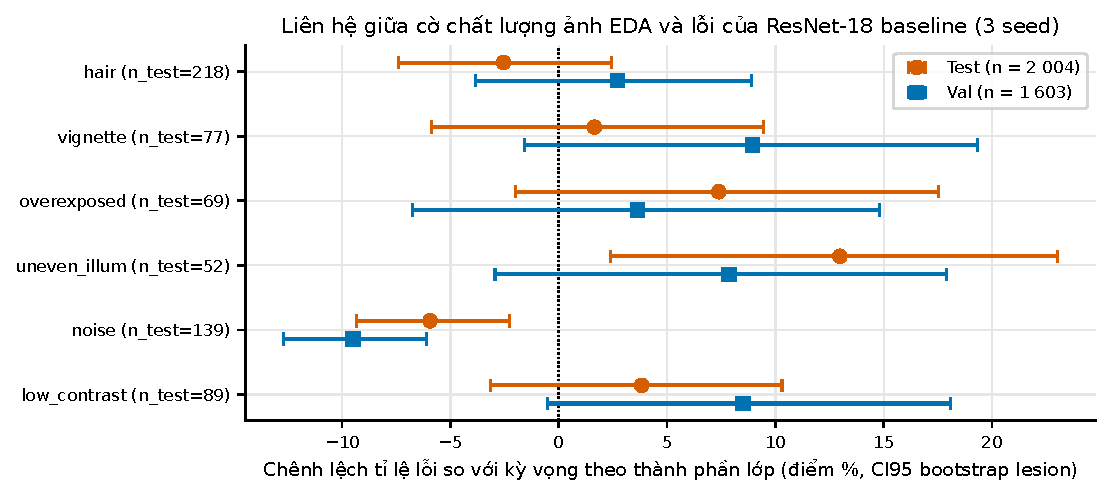
\includegraphics[width=0.95\linewidth]{figures/eda_cnn_link.pdf}
\vspace{2pt}
\scriptsize
\begin{itemize}
    \item \textbf{Cặp nhầm số 1:} \texttt{mel}$\rightarrow$\texttt{nv} ($0{,}311$, TB $69{,}0/222$ ảnh) do chồng lấn sắc tố ở $224{\times}224$.
    \item \textbf{Nhóm ảnh khó:} $\approx 8\%$ ảnh test sai ở cả 3 seed (chủ yếu ca không điển hình của \texttt{mel, df, akiec}).
    \item \textbf{Chuẩn hóa theo lớp:} \emph{Sáng không đều} \& \emph{quá sáng} có lỗi cao hơn kỳ vọng; cờ \emph{nhiễu} lỗi thấp do gắn nguồn \texttt{follow\_up} (\texttt{nv}).
\end{itemize}
\end{column}
\end{columns}
\end{frame}

% Slide 13
\begin{frame}{2.8 Hệ thống Demo Tương tác Streamlit (\texttt{app.py})}
\begin{columns}[T,onlytextwidth]
\begin{column}{0.52\textwidth}
\footnotesize
\begin{block}{Kiến trúc 3 Tab trực quan \& An toàn}
\begin{enumerate}
    \item \textbf{Tab 1 -- QC \& Dự đoán:} Chạy trực tiếp 6 bộ dò EDA, cảnh báo cờ vượt ngưỡng, so sánh xác suất 7 lớp của \texttt{baseline\_seed42.pt} (khớp \textbf{20/20} nhãn kiểm thử).
    \item \textbf{Tab 2 -- Từng giai đoạn \& Stress Test:} Chuỗi ảnh qua từng phép xử lý, bản đồ $|\text{sau}-\text{trước}|$, $\Delta E_{76}$, mask Otsu/lông, histogram FOV \& thanh trượt giả lập suy giảm 2.5c.
    \item \textbf{Tab 3 -- Grad-CAM \& Bảng số liệu:} Nội suy Grad-CAM \texttt{layer4}, đo \% năng lượng chú ý trong tổn thương vs lông.
\end{enumerate}
\end{block}
\end{column}
\begin{column}{0.45\textwidth}
\centering
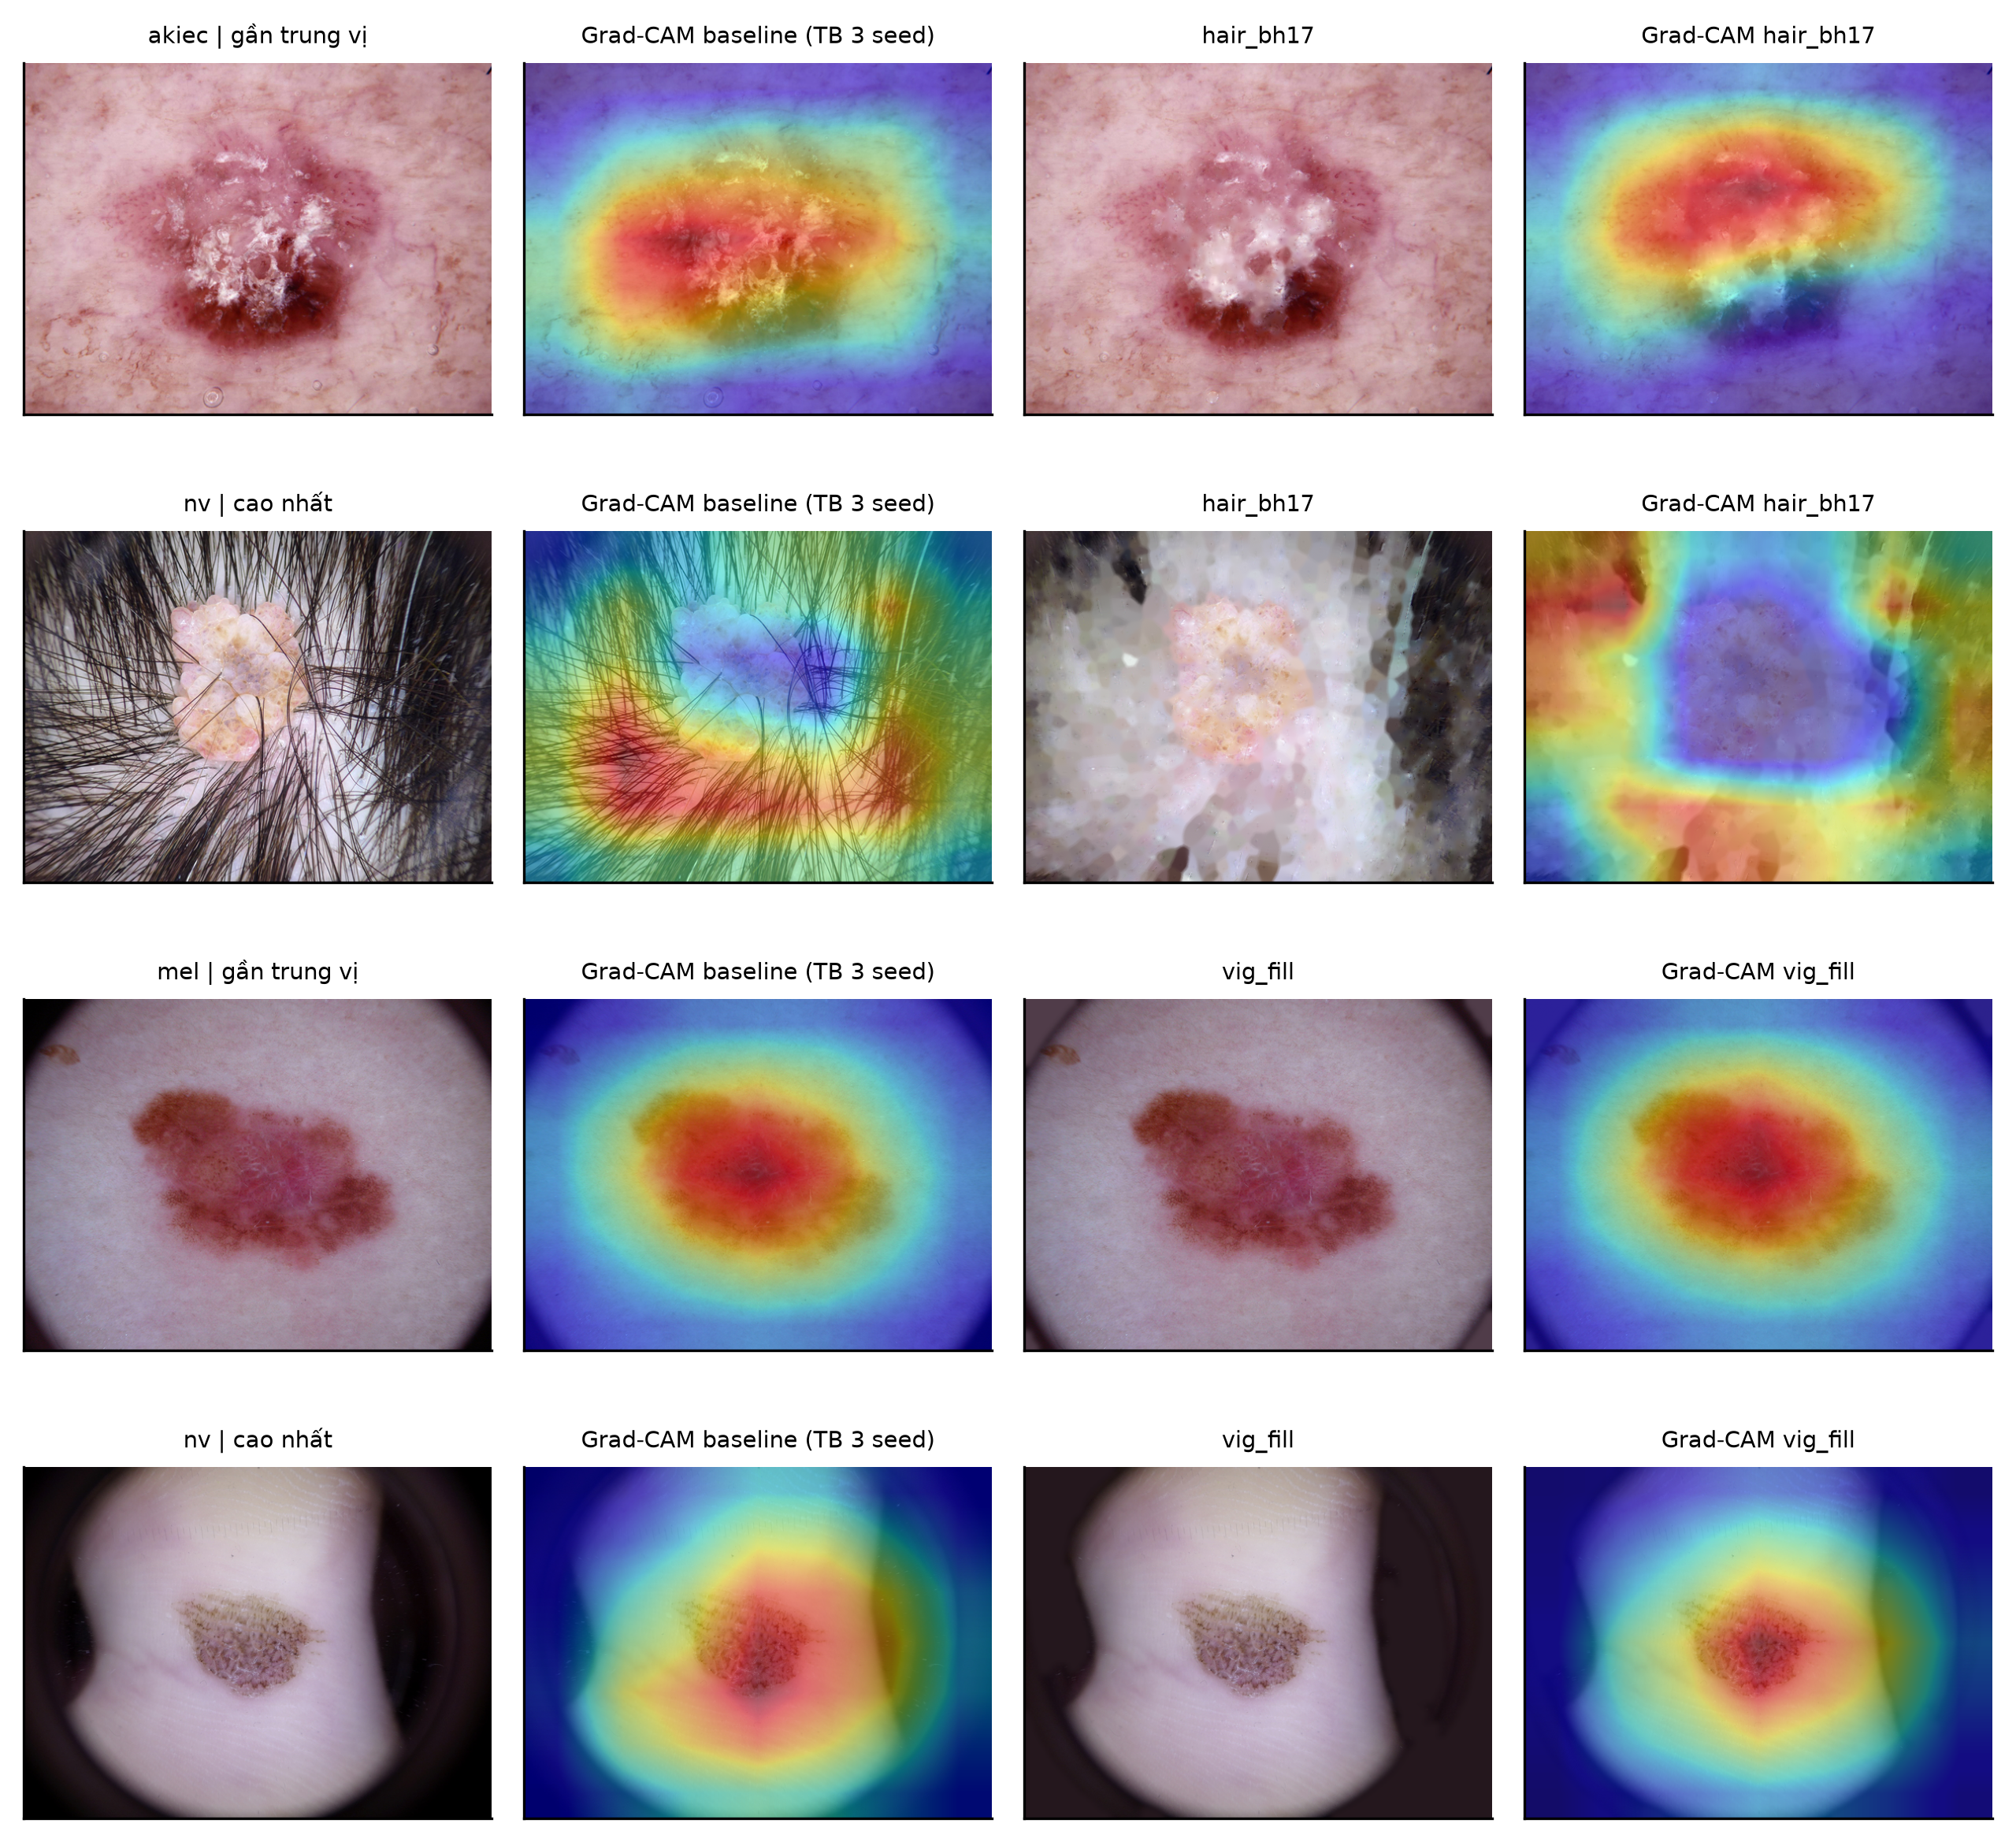
\includegraphics[height=0.68\textheight,keepaspectratio]{figures/impact_d3_grid.png}
\end{column}
\end{columns}
\end{frame}

% Slide 14
\begin{frame}{3. Kết luận, Hạn chế, Phân công \& Khai báo AI}
\begin{columns}[T,onlytextwidth]
\begin{column}{0.53\textwidth}
\footnotesize
\begin{block}{Tổng kết đóng góp}
\begin{itemize}
    \item Chứng minh thực nghiệm trên 51 lượt train ResNet-18 + 6 lượt khảo sát kiến trúc: CNN fine-tune tự thích nghi tốt trên ảnh dermoscopy chuẩn; biến đổi toàn cục/đại trà dễ xóa tín hiệu chẩn đoán.
    \item Giải mã trọn vẹn cơ chế qua 4 tầng phân tích \& đề xuất pipeline 2 nhánh (QC + CNN) trung thực với số liệu.
\end{itemize}
\end{block}
\vspace{2pt}
\scriptsize
\textbf{Hạn chế \& Hướng mở:} 1 split $\times$ 3 seed; mask Otsu/black-hat thô (lỗi trên rìa tối \& lông bạc); hướng mở dùng U-Net segmentation, color constancy Chương 4 và Focal Loss.
\end{column}
\begin{column}{0.45\textwidth}
\resizebox{\linewidth}{!}{%
\begin{tabular}{lll}
\toprule
\textbf{Thành viên} & \textbf{MSV} & \textbf{Phụ trách chính} \\
\midrule
Nguyễn Trung Nam & B23DCVT299 & Run L40S, 3 CNN, 2.5c, Demo, PDF \\
Phan Nguyễn Việt Dũng & B23DCCN210 & Khung train, 2.1--2.4, 2.5a, 2.5c \\
Lê Duy Anh & B23DCCN026 & Lý thuyết \& BC Mở đầu, 2.5a \\
Đinh Khánh Sơn & B23DCDT223 & EDA 2.2, 2.5b, lỗi 2.8, Demo \\
Đào Phạm Bích Ngọc & B23DCVT308 & Hình thái Ch.7, 2.5b, 2.6--2.7, Slide \\
\bottomrule
\end{tabular}%
}
\vspace{4pt}
\begin{block}{Khai báo AI minh bạch}
\tiny AI hỗ trợ viết khung mã nguồn, biểu đồ, UI \texttt{app.py} và chế bản LaTeX. Nhóm trực tiếp thiết kế giả thuyết, chạy thực nghiệm HAM10000, kiểm tra trực quan mask/ảnh lỗi và đối soát 100\% con số từ \texttt{outputs/}.
\end{block}
\end{column}
\end{columns}
\end{frame}

\end{document}
